% This is "sig-alternate.tex" V2.1 April 2013
% This file should be compiled with V2.5 of "sig-alternate.cls" May 2012
%
% This example file demonstrates the use of the 'sig-alternate.cls'
% V2.5 LaTeX2e document class file. It is for those submitting
% articles to ACM Conference Proceedings WHO DO NOT WISH TO
% STRICTLY ADHERE TO THE SIGS (PUBS-BOARD-ENDORSED) STYLE.
% The 'sig-alternate.cls' file will produce a similar-looking,
% albeit, 'tighter' paper resulting in, invariably, fewer pages.
%
% ----------------------------------------------------------------------------------------------------------------
% This .tex file (and associated .cls V2.5) produces:
%       1) The Permission Statement
%       2) The Conference (location) Info information
%       3) The Copyright Line with ACM data
%       4) NO page numbers
%
% as against the acm_proc_article-sp.cls file which
% DOES NOT produce 1) thru' 3) above.
%
% Using 'sig-alternate.cls' you have control, however, from within
% the source .tex file, over both the CopyrightYear
% (defaulted to 200X) and the ACM Copyright Data
% (defaulted to X-XXXXX-XX-X/XX/XX).
% e.g.
% \CopyrightYear{2007} will cause 2007 to appear in the copyright line.
% \crdata{0-12345-67-8/90/12} will cause 0-12345-67-8/90/12 to appear in the copyright line.
%
% ---------------------------------------------------------------------------------------------------------------
% This .tex source is an example which *does* use
% the .bib file (from which the .bbl file % is produced).
% REMEMBER HOWEVER: After having produced the .bbl file,
% and prior to final submission, you *NEED* to 'insert'
% your .bbl file into your source .tex file so as to provide
% ONE 'self-contained' source file.
%
% ================= IF YOU HAVE QUESTIONS =======================
% Questions regarding the SIGS styles, SIGS policies and
% procedures, Conferences etc. should be sent to
% Adrienne Griscti (griscti@acm.org)
%
% Technical questions _only_ to
% Gerald Murray (murray@hq.acm.org)
% ===============================================================
%
% For tracking purposes - this is V2.0 - May 2012

\documentclass{sig-alternate-05-2015}

\usepackage{amsmath}
\usepackage{listings}
\usepackage{color}

\definecolor{codegreen}{rgb}{0,0.6,0}
\definecolor{codegray}{rgb}{0.5,0.5,0.5}
\definecolor{codepurple}{rgb}{0.58,0,0.82}
\definecolor{backcolour}{rgb}{0.95,0.95,0.92}
 
\lstdefinestyle{mystyle}{
    backgroundcolor=\color{backcolour},   
    commentstyle=\color{codegreen},
    keywordstyle=\color{codegreen},
    numberstyle=\tiny\color{codegray},
    stringstyle=\color{codepurple},
    basicstyle=\ttfamily\small,
    breakatwhitespace=false,         
    breaklines=true,                 
    captionpos=b,                    
    keepspaces=true,                                 
    showspaces=false,                
    showstringspaces=false,
    showtabs=false,                  
    tabsize=2
}
 
\lstset{style=mystyle}

\begin{document}

% Copyright
% \setcopyright{acmcopyright}
%\setcopyright{acmlicensed}
%\setcopyright{rightsretained}
%\setcopyright{usgov}
%\setcopyright{usgovmixed}
%\setcopyright{cagov}
%\setcopyright{cagovmixed}


% DOI
% \doi{10.475/123_4}

% ISBN
% \isbn{123-4567-24-567/08/06}

%Conference
% \conferenceinfo{PLDI '13}{June 16--19, 2013, Seattle, WA, USA}

% \acmPrice{\$15.00}

%
% --- Author Metadata here ---
% \conferenceinfo{WOODSTOCK}{'97 El Paso, Texas USA}
%\CopyrightYear{2007} % Allows default copyright year (20XX) to be over-ridden - IF NEED BE.
%\crdata{0-12345-67-8/90/01}  % Allows default copyright data (0-89791-88-6/97/05) to be over-ridden - IF NEED BE.
% --- End of Author Metadata ---

\title{{\ttlit Test Case Generation} and {\ttlit Symbolic Execution} using 
Z3\titlenote{Z3 is a high-performance theorem prover. More information about Z3 is
available at \texttt{https://github.com/Z3Prover/z3/wiki}}}
\subtitle{Project Report
\titlenote{This report is part of the project work for \textit{Automated Software Engineering}
course instructed by Dr. Taylor Johnson in Fall, 2015.}}
%
% You need the command \numberofauthors to handle the 'placement
% and alignment' of the authors beneath the title.
%
% For aesthetic reasons, we recommend 'three authors at a time'
% i.e. three 'name/affiliation blocks' be placed beneath the title.
%
% NOTE: You are NOT restricted in how many 'rows' of
% "name/affiliations" may appear. We just ask that you restrict
% the number of 'columns' to three.
%
% Because of the available 'opening page real-estate'
% we ask you to refrain from putting more than six authors
% (two rows with three columns) beneath the article title.
% More than six makes the first-page appear very cluttered indeed.
%
% Use the \alignauthor commands to handle the names
% and affiliations for an 'aesthetic maximum' of six authors.
% Add names, affiliations, addresses for
% the seventh etc. author(s) as the argument for the
% \additionalauthors command.
% These 'additional authors' will be output/set for you
% without further effort on your part as the last section in
% the body of your article BEFORE References or any Appendices.

\numberofauthors{1} %  in this sample file, there are a *total*
% of EIGHT authors. SIX appear on the 'first-page' (for formatting
% reasons) and the remaining two appear in the \additionalauthors section.
%

\author{
% You can go ahead and credit any number of authors here,
% e.g. one 'row of three' or two rows (consisting of one row of three
% and a second row of one, two or three).
%
% The command \alignauthor (no curly braces needed) should
% precede each author name, affiliation/snail-mail address and
% e-mail address. Additionally, tag each line of
% affiliation/address with \affaddr, and tag the
% e-mail address with \email.
%
% 1st. author
\alignauthor
Shafiul Azam Chowdhury\\
       \affaddr{Department of Computer Sc. and Engineering}\\
       \affaddr{The University of Texas at Arlington}\\
       \email{shafiulazam.chowdhury@mavs.uta.edu}
}


\maketitle
\begin{abstract}
This project aims at demonstrating interesting usage of automated software 
engineering tools. \textit{Z3} is an efficient theorem prover \cite{DeMoura:Z3} which can be used 
for automated \textit{test case generation} of \textit{transition systems} and 
performing \textit{symbolic execution} \cite{King:SE} of computer programs. I have addressed these two aspects 
of automated software engineering in this project. The first task finds test cases for 
a small-sized multi-state transition system. The second task encodes two interesting 
computer programs in their \textit{Static Single Assignment (SSA)} \cite{Alpern:SSA} forms 
and utilizes Z3 for performing symbolic execution. I perform static analysis on a 
small computer program for finding interesting inputs automatically and demonstrate 
automatic bug-finding for an iterative version of the \textit{quicksort} algorithm. 
\end{abstract}


\keywords{Automated software engineering; static analysis; test case generation}

\section{Introduction}
In this project I address two different automated software engineering problems. In the first task I generate \textit{test cases} automatically for a transition system. This task demonstrates powerful usage of a state of-the art SMT solver; one can use this tool for finding interesting test cases automatically for a transition system. I modeled the popular ``n-puzzle'' game specifying its initial states and transition relations. This multi-state game is ideal for modeling transition relations and safety or liveness requirements. The game begins with one initial state and after some transitions reach a specific goal state. One sort of test case generation problem for this system is finding those \textit{initial} states from which we can reach the goal state after exactly \textit{x} number of transitions.

I present symbolic execution of interesting computer programs in the second task, which is further organized in two sub tasks. In the first sub-task I analyze a program using symbolic execution to find what inputs cause certain paths of the program to be executed. The second task demonstrates automatic bug finding by encoding a computer program \textit{(quicksort for my project)} into \textit{Static Single Assignment (SSA)} form and negating some assertion statements. Z3 the SMT solver can then be utilized to determine if the encoding is satisfiable indicating the system is buggy indeed. By harnessing such static analysis techniques we can perform various automated software engineering tasks in similar projects.

In both of these tasks, I have used Z3's Python API (also known as Z3Py). Z3 is an efficient SMT solver \cite{DeMoura:Z3} developed at Microsoft Research. Z3Py enables us to utilize the powerful features of Z3 in the very popular programming platform - Python. Z3Py can be downloaded from their website at \texttt{https://github.com/Z3Prover/z3}.

\section{Test Case Generation for transition systems}

This section describes first task of the project in details. I begin
with presenting a definition of \textit{transition systems} and our
specific problem \textit{n-puzzle} as a transition system. We also
define the task definition that is what do we mean by \textit{test 
case generation}. Next, we focus on creating a formal model of the 
system. A good approach is to first formalize some requirements
of the system which helps identifying the state variables required
to model the system. I then formalize all transition formulae for 
the system. We are then in a position to start implementing the
test case generation problem using Z3Py.

My contribution for this task is an application written in Python 
(which uses Z3 API). The application is complete and parameterized.
The application creates graphical output for the \textit{n-puzzle}
problem, a useful visual aid which demonstrates all of the states
of a game round\footnote{Graphical output is only available when the 
problem is satisfiable i.e. test cases really exist for given parameters.}.  

\subsection{{\subsecit N-puzzle} and transition systems}

We start with an introduction of the n-puzzle game. A more specific 
example would be \textit{15 puzzle} game, which 
consists of a frame of numbered square tiles in random order 
with one tile missing \cite{wiki:npuzzle}. In the 15-puzzle game, these
numbers can any of the numbers from 1 to 15. We say that the board 
has 16 \textit{cells}. No two cell can have the same number. The final
(or goal) state of the game is where the first cell has the number 1,
the second cell has the number 2, and so on. The empty cell should
be at the sixteenth cell. Final state of a 15-puzzle game is shown
in Figure \ref{fig:npfinal}. 

\begin{figure}
\centering
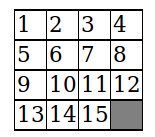
\includegraphics{npfinal}
\caption{Final state of a 15-puzzle game.}
\label{fig:npfinal}
\end{figure}

A game round starts with a \textit{initial} state where cells may have
any values other than the values cell have in the final state. 
After a certain number of \textit{rounds}, the game may go into 
the final state. At any of these rounds, only the empty cell 
is allowed to swap its position with one of its adjacent cells. 
That is, the at each round the empty cell can move only in any the  
upwards, downwards, left of right directions. No other movement of 
cell is allowed. Once the game has reached in the final state, no 
further transitions (movement of the empty cell) are allowed.

Now we are in a position to define the task specifically. Given 
a fixed size of the n-puzzle board, we want to automatically find 
the initial cases from which one may reach the final state making only
\textit{x} transitions. Thus my task falls into the category of test case 
generation problem, where one has to convert the system model into SAT/SMT 
problem and utilize an SMT solver for determining satisfiability.

I chose \textit{n-puzzle} as it is very suitable for modeling in the scope of 
a short-term project. Later I show that this problem falls into the category 
of transition systems, for which we have formal definitions of modeling. A 
transition system has a finite set of typed state variables, a set of initial 
states and a transition description of transitions between states \cite{Alur:CPS}. 

\subsection{Writing System Specifications}
When modeling a transition system, one can start with identifying the state 
variables required for the system and then formalize some of the system's 
requirements. The problem with this approach is, one may end up with unnecessary 
and/or unimportant variables. The alternative is to try formalizing the specifications
first and identify state variables on demand. This approach helps eliminating 
unnecessary vaiables by not creating them at the first time. 

For this reason, we start up with some of the system specifications for \textit{8-puzzle}:

\begin{itemize}
  \item At any state, any cell should have a value greater than 0 and less than or equal to 9.
  We represent the empty cell by the value 9 (16 in a 15-puzzle variant).
  \item No two cell may have the same value.
  \item Only in the final state the cells should have their values ordered, and the system 
  stays in its final round as soon as it reaches there.
\end{itemize}

Once we have identified these specifications, we can determine possible state variables. 
We immediately identifiy that we need one integer variable per cell to keep track which 
number it is representing. Also, we might need a \textit{mode} variable to represent goal 
and non-goal states.

\subsection{Modeling the transition system}

In this section we describe our modeling approach for the transition system. We begin with 
defining some of the transition formulae, and then proceed by specifying implementatio details.

\subsubsection{Transition relations}

Once we have identified possible state variables, we can start defining transition relations. 
For example, for each of the non-goal states, equation \ref{eq:1} represents the transition 
relation showing important constraints, along with other constrains (not shown) to enfore 
system requirements. In the equation, $ cell_i $ represents the value (number) represented by
that cell at step $ i $; $ cell_{i+1} $ represents that cell's value in the next step. $ E $ 
is a symbol for representing the empty cell, which is represented by the number $ 9 $ in a 
$ 3 X 3 $ board. In equation \ref{eq:1}, we represent the right adjacent cell of current cell 
by $ e_{i} $ (``e'' can be considered as shorthand for ``east''). We represent the bottom, left and up 
adjacent cells of the current cell by the symbols $ s_i $, $ w_i $ and $ n_i $ resectively. 
 
\begin{multline} \label{eq:1}
(cell_i = E \wedge \\
  (cell_{i+1} = e_{i} \wedge e_{i+1} = E) \vee \\
  (cell_{i+1} = w_{i} \wedge w_{i+1} = E) \vee \\
  (cell_{i+1} = n_{i} \wedge n_{i+1} = E) \vee \\
  (cell_{i+1} = s_{i} \wedge s_{i+1} = E) \\
))  \vee \\
(
  cell_i != E \wedge ( \\
    (e_{i} = E \wedge e_{i+1} = cell_{i} \wedge cell_{i+1} = E) \vee \\
    (w_{i} = E \wedge w_{i+1} = cell_{i} \wedge cell_{i+1} = E) \vee \\
    (n_{i} = E \wedge n_{i+1} = cell_{i} \wedge cell_{i+1} = E) \vee \\
    (s_{i} = E \wedge s_{i+1} = cell_{i} \wedge cell_{i+1} = E) \vee \\
    (cell_{i+1} = cell_{i})
  )
)
\end{multline}

It should be noted that we have not mentioned all of the required constraints in equation \ref{eq:1}. 
For example, this equation is not applicable directly if current cell is one of the first three cells 
in a $3 X 3$ board, since $n_{i+1}$ represents the top adjacent cell of current cell which is not 
applicable here. We also have not shown other system requirements. For example, in a $3 X 3$ board each 
cell should have one of these values arbitrarily from 1 to 9, and no two cells should have the same 
value. Also note that the value 9 represents the empty cell. 

\subsubsection{Implementation details}

We have used Z3's Python API for modeling the transition system. As mentioned previously, we need one 
integer variable for each of the cells. However, using \textit{Bit-Vectors\footnote{Machine arithmetic 
is available in Z3Py as Bit-Vectors.}} instead of integers is recommended as it reduces runtime. Also, 
we need to track value of each cell in each of the steps of the system. We model this requirement using 
\textit{Functions} feature of the Z3Py API. For each cell, we now have one function which takes one 
integer (Bit-Vector) as input and returns one integer (Bit-Vector) as output. the input integer denotes 
the current step, and the output integer denotes value of that cell at that step.

Finally, instead of using a python list to hold the nine functions for each of the nine cells, we use
a two dimensional python list as it enables us to access the cells easily by mentioning two 
indices - representing the ``row'' index and ``column'' index of the cell. The entire model 
is written inside a python class which takes three arugments in its constructor. The first 
argument represents the board size, the second argument denotes number of steps \textit{ (i.e. 
in how many steps we need to reach the goal state)} and the final one puts a bound on how 
many test cases are needed to be generated.


\subsection{Model analysis}

In this section we analyse our implementation of the n-puzzle transition system. We generate 
graphical result showing not only the initial step, but each of the subsequent 
steps of a game round. We generate as many test cases as requested (given such number of test 
cases are available). One such graphical output is presented in Figure \ref{fig:npdemo} where 
the board size is $4 X 4$, two test cases are requested, and the goal state is reached 
in exactly 5 steps.

\begin{figure}
\centering
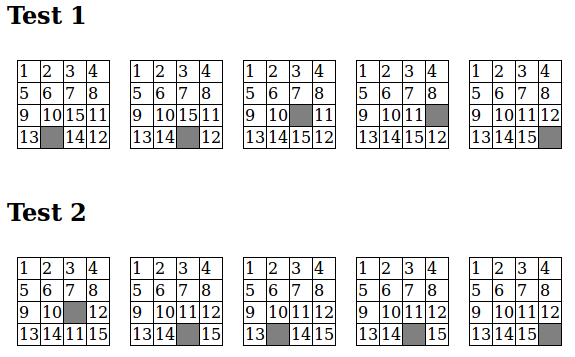
\includegraphics[width=3in]{npdemo}
\caption{Sample result of our implementation of the n-puzzle system. Two test cases
are displayed for a 4X4 board, where the goal state is reached in exactly 5 steps.}
\label{fig:npdemo}
\end{figure}

\section{Symbolic execution using Z3}

In this section I present \textit{symbolic execution} of computer programs using 
Z3's Python API. Before explaining the definition of symbolic execution, i discuss 
the motivating task descriptions. I selected two different computer programs for this 
section of my project. Each of the tasks have limited scope well suited for the 
project but demonstrates interesting software engineering challenges. They also 
exhibit powerful usage of Z3. My contribution in this section is encoding 
two computer problems into \textit{static single assignment (SSA)} form and 
developing a library for easily encoding common programming tasks.

\subsection{Task A: Automatic Input Finding} \label{taskA}

My first sub-task for symbolic execution is finding inputs automatically for a 
small sized program (see Listing \ref{lst:lottery}). This program has three 
integer input variables which may accept different value. Based on values of 
each of these three inputs, the final goal is to calculate a wining number and 
check if that number matches with a pre-defined number. Our goal is to find values 
of the input variables automatically, for which the final \texttt{if} condition 
evaluates to true. One way to accomplish this could be executing the program many 
times, each times with different values for the inputs randomly chosen, which however, 
may fail to accomplish the goal. Our approach will be finding the inputs automatically 
leveraging static analysis techniques, without even executing the code.

This problem is a slightly modified version of laboratory assignment\footnote{Available: 
\texttt{https://www.ida.liu.se/~TDDC90/labs/}} offered at \textit{DDC90 Software Security} course\cite{online:tddc}.

\lstinputlisting[language=C, caption={Sample program for input finding task}, label={lst:lottery}]{lottery.c}

\subsubsection{Symbolic execution overview}

Now that I have presented the task definition, I will discuss symbolic execution in this 
section. For my task, I would like to find the inputs automatically for which the 
program takes a particular execution path. Instead of executing the program, it is 
``symbolically'' executed for a set of \textit{classes} of inputs \cite{King:SE}. 
For illustration, the variables \texttt{a}, \texttt{b} and \texttt{c} will be replaced by 
``symbols'' instead of having any concrete value. We turn the entire program into SMT problem 
and ask Z3 to check whether it is satisfiable. If satisfiable, Z3 returns a model denoting 
possible values for each of the inputs. 

\subsubsection{Modeling challenges} \label{modeling_challenges}

I demonstrate some modeling challenges in this section. Consider a sample program 
listed in Listing \ref{lst:achallenge}. If we naively encode this program into 
$ result=0 \wedge ... \wedge result=1 $, the SMT solver will simply return unsatisfiable. 
What we need is to use static single assignment form \cite{Alpern:SSA} where each time a 
variable is assigned to a new value, we need another new variable for it's SMT encoding. 
For the code listed in Listing \ref{lst:achallenge}, we need an encoding like 
$ result_0 = 0 \wedge ... \wedge result_1 = result_0 + 1 $.

\begin{lstlisting}[caption={Sample program showing modeling challenges for Task A}, label={lst:achallenge}]
int result =0;
...
result = result + 1;
\end{lstlisting}

\subsubsection{Model analysis}

I developed two models for this subtask defined in section \ref{taskA}. The first model encode only 
specific branches of the given program\footnote{Available: \texttt{lottery.c} file in project 
artifacts}: the path corresponding to the ``then" followed by the ``else" 
followed by the ``then", and the ``else" followed by the ``then" followed by the `else". Encoding 
these paths, we ask Z3 to find any satisfiable models i.e. are there any input values for which 
we ``win the lottery". In the second model, I have encoded all the paths and queried Z3 similarly. 
To find these models, please see section \ref{artifacts}.


\subsection{Task B: Bug Finding using Static Analysis}

In this subtask I demonstrate how static analysis can be used for automated bug finding. 
Automated bug finding is crucial as by the  fact  that  programmers  often do  not  take  the
time  to  write  detailed  specifications \cite{Hangal:2002}. Techniques like sophisticated 
program analysis is valuable for automatically finding bugs in software \cite{Hovemeyer:2004}. 
Often program correctness is enforced by placing \texttt{assert} statements in the code, which 
describes some expected behavior of the code at that point. One bug finding strategy would be 
encoding the program into SSA form with it's \texttt{assert} conditions negated and asking SMT 
solvers whether there exists any satisfiable model. If there exists any - we have found a bug 
in our program. 

\subsubsection{An example demonstrating bug finding strategy}

In this section I present a small example demonstrating my bug finding approach. Consider the 
program listed in Listing \ref{lst:bexample} which have an assert statement. I encode the program 
into SSA form in Listing \ref{lst:bencoding}, where the assert statement is negated. Now Z3 can 
be asked to check whether the problem is satisfiable. If yes, we know that the program does not 
behave as expected.

\begin{lstlisting}[caption={Dummy program for Task B}, label={lst:bexample}]
int compute(int a, int b){
int result =0;

if((a % 5) != (b % 7)){

result = a + 1;
assert(result == b);

}
...
\end{lstlisting}

\begin{lstlisting}[caption={Target encoding for Task B}, label={lst:bencoding}]
(declare-const a0 Int)
(declare-const b0 Int)
(declare-const result0 Int)
(assert (= result0 0))
(assert (not (= (mod a0 5)
(mod b0 7))))
(declare-const result1 Int)
(assert (= result.SSA1 (+ a0 1)))
(assert (!= result1 b0))
(check-sat)
(get-model)
\end{lstlisting}

\subsubsection{Modeling a {\subsecit quicksort} algorithm}

I chose an iterative version\footnote{Available in submitted artifacts.} of the 
\textit{quicksort} algorithm as it offers interesting encoding challenges 
including encoding loops and arrays, and yet fits well into the project scope. In this 
section I briefly discuss some implementation details and some challenges faced.

Like my \textit{n-puzzle} problem encoding, I have used Z3's \textit{Bit-Vectors} feature 
for encoding integers. An array can be easily encoded using a \textit{function} which takes 
one Bit-Vector as input and returns one Bit-Vector as output. Then, the argument can be used 
for mimicking the array select operation. However, as we need multiple 
versions for a single array (each time an array is updated, we need a new variable to represent
it, as discussed in section \ref{modeling_challenges}), we use a function 
which takes two arguments (two Bit-Vectors) instead of one argument. The first argument 
is for specifying which version of the array we need, and the second version works as 
an index for accessing array elements. 

Once we start converting our quicksort program using this strategy, we quickly end up with 
lots of repeated code. For example each time we need to swap two elements in the array, we 
need to write as many code (in fact, more than this amount!) as listed in Listing \ref{lst:bswap}. 
Similarly, one need to write tons of repeated code for common functionalities like initiating 
arrays and integers, incrementing (decrementing) integers, accessing array elements etc. I 
developed a small library\footnote{Available in \texttt{helper.py} file within submitted artifacts.} which 
offers keeping track of different versions of variables in their SSA form automatically and 
encoding common operations 
just mentioned. For example, without manually creating multiple versions for an array, one can just 
write \texttt{arr = encode\_array('arr', init\_val=[3, 2, 1])} to create an integer array with 
initial values \texttt{{3, 2, 1}}. \texttt{arr.c} then gives us the current version of this array 
in the SSA form. We can then call \texttt{arr.u(top.c, 5} to update the element at index 
\texttt{top} to value 5. Some similar operations are shown in Listing \ref{lst:bfeatures}.

\lstinputlisting[language=Python, caption={Code required for encoding swapping two elements of an array}, label={lst:bswap}]{bswap.py}

\begin{lstlisting}[caption={Sample library usage for encoding common programming functionalities}, label={lst:bfeatures}]
# int a[] = {3, 2, 1};
arr = encode_array('arr', init_val=[3, 2, 1])

# int p = 0;
p = encode_int('p', init_val=0)

# p = (p + 1);
p.plusplus()

# swap (&arr[p], &arr[h]);
arr.swap(p.c, h.c)
\end{lstlisting}

\subsubsection{Model analysis}

I developed a complete encoding of the quicksort algorithm using Z3's Python API. My main 
contribution is developing a reusable helper library which provides handy encoding 
functionalities for programs having simple types and arrays, loops and branches. The helper 
library functions reduce duplicate code a lot and automatically keeps track of all 
versions of each variable in SSA form. Most of the functions of this library produces 
encoding for both \texttt{if-then} and \texttt{if-else} branches. For example, suppose we 
are encoding a sample code where an array gets updated only in \texttt{if-then} branch. My 
library produces encoding which satisfies this requirement, i.e. next version of the 
array will be updated only inside \texttt{if-then} branch and will remain unchanged inside 
\texttt{if-else} branch.

Using our helper library, I encoded the quicksort algorithm along with bug finding assertion, 
negated. For my bug finding approach, I used following encoding: each array element is greater 
than next array element after quicksort algorithm sorts the array in ascending order. Satisfiable 
answer from Z3 will indicate possible bug in the program. However, in our case the encoding was 
unsatisfiable, which means no possible bug was found. 

There is another possible usage of my application: instead of finding bugs, one can give an arbitrary array 
as input to my program and run it to view each version of the array. Such an usage 
can be used for demonstration purposes, e.g. for demonstrating how quicksort algorithm sorts a given array.

% \subsection{Tables}
% Because tables cannot be split across pages, the best
% placement for them is typically the top of the page
% nearest their initial cite.  To
% ensure this proper ``floating'' placement of tables, use the
% environment \textbf{table} to enclose the table's contents and
% the table caption.  The contents of the table itself must go
% in the \textbf{tabular} environment, to
% be aligned properly in rows and columns, with the desired
% horizontal and vertical rules.  Again, detailed instructions
% on \textbf{tabular} material
% is found in the \textit{\LaTeX\ User's Guide}.

% Immediately following this sentence is the point at which
% Table 1 is included in the input file; compare the
% placement of the table here with the table in the printed
% dvi output of this document.

% \begin{table}
% \centering
% \caption{Frequency of Special Characters}
% \begin{tabular}{|c|c|l|} \hline
% Non-English or Math&Frequency&Comments\\ \hline
% \O & 1 in 1,000& For Swedish names\\ \hline
% $\pi$ & 1 in 5& Common in math\\ \hline
% \$ & 4 in 5 & Used in business\\ \hline
% $\Psi^2_1$ & 1 in 40,000& Unexplained usage\\
% \hline\end{tabular}
% \end{table}

% To set a wider table, which takes up the whole width of
% the page's live area, use the environment
% \textbf{table*} to enclose the table's contents and
% the table caption.  As with a single-column table, this wide
% table will ``float" to a location deemed more desirable.
% Immediately following this sentence is the point at which
% Table 2 is included in the input file; again, it is
% instructive to compare the placement of the
% table here with the table in the printed dvi
% output of this document.


% \begin{table*}
% \centering
% \caption{Some Typical Commands}
% \begin{tabular}{|c|c|l|} \hline
% Command&A Number&Comments\\ \hline
% \texttt{{\char'134}alignauthor} & 100& Author alignment\\ \hline
% \texttt{{\char'134}numberofauthors}& 200& Author enumeration\\ \hline
% \texttt{{\char'134}table}& 300 & For tables\\ \hline
% \texttt{{\char'134}table*}& 400& For wider tables\\ \hline\end{tabular}
% \end{table*}
% end the environment with {table*}, NOTE not {table}!

\section{Project Artifacts} \label{artifacts}

This section briefly explains each of the artifacts submitted in this project 
and the location they are available in.


\section{Conclusions}

In this project I demonstrate powerful usage of Z3 - an efficient SMT 
solver in two different automated software engineering tasks. First task 
is a \textit{test case generation} problem where I automatically 
generate \textit{initial} states of a popular sliding game (n-puzzle). 
From each of these different initial states one can reach the final state 
only after \textit{x} number of transitions. My approach considers the 
game as a transition system and define its state variables, initial states 
and transition relations, along with some specifications. My entire project 
is parameterized and it generates output in HTML form, which can be viewed 
in any web browser.

In the second part of the project I demonstrate symbolic execution using Z3. 
I applied this static analysis technique for automatically finding inputs of 
a program having multiple \texttt{if-then-else} execution branches. I then encode an 
iterative \textit{quicksort} algorithm into SSA form and utilize Z3's Python 
API for finding bugs in the algorithm provided. I have developed a small 
but helpful helper library for encoding common programming codes. 
This library can be reused in future projects and can be extended easily as 
well. One limitation of the project is we perform the encoding manually i.e. 
we do not parse the given program automatically. This issue can be addressed in 
future work so that we can automatically encode computer programs into their 
SSA forms and find bugs in them.


%\end{document}  % This is where a 'short' article might terminate

%ACKNOWLEDGMENTS are optional
\section{Acknowledgments}
I am grateful to my course instructor, \textit{Dr. Taylor T. Johnson} for 
his inspiration and helpful advices regarding the project. I would also like to thank my 
classmates who provided valuable help and support throughout the coursework.

%
% The following two commands are all you need in the
% initial runs of your .tex file to
% produce the bibliography for the citations in your paper.
\bibliographystyle{abbrv}
\bibliography{sigproc}  % sigproc.bib is the name of the Bibliography in this case
% You must have a proper ".bib" file
%  and remember to run:
% latex bibtex latex latex
% to resolve all references
%
% ACM needs 'a single self-contained file'!
%
%APPENDICES are optional
%\balancecolumns
% \appendix
%Appendix A

%\balancecolumns % GM June 2007
% That's all folks!
\end{document}
